\documentclass[a4paper,14pt,russian]{report}
\usepackage[utf8]{inputenc}
\usepackage[T2A]{fontenc}
\usepackage{amsmath}
\usepackage{listings}
\usepackage{xcolor}
\usepackage{tabularx}
\usepackage{geometry}
\usepackage{tikz}
\usepackage{titlesec}
\usepackage{extsizes}
\usepackage{graphicx}
\usepackage{extsizes}
\usepackage{amsmath}
\usepackage{listings}
\usepackage{xcolor}
\usepackage{tabularx}
\usepackage{geometry}
\usepackage{titlesec}
\usepackage[font=small,labelfont=bf]{caption}
\usepackage{indentfirst}

\usetikzlibrary{shapes,arrows}
\tikzstyle{line} = [draw, -latex']
\tikzstyle{decision} = [
  diamond,
  aspect=3,
  draw,
  fill=yellow!20,
  % text width=5em,
  text badly centered,
  node distance=2cm,
  % inner sep=0pt
]
\tikzstyle{process} = [
  rectangle,
  draw,
  fill=blue!20,
  node distance=2cm,
  % text width=10em,
  text centered,
  minimum height=3em
]
\tikzstyle{terminal} = [
  rectangle,
  draw,
  fill=red!20,
  node distance=2cm,
  text width=5em,
  text centered,
  minimum height=3em,
  rounded corners
]
\tikzstyle{io} = [
  trapezium,
  trapezium left angle=120,
  trapezium right angle=60,
  draw,
  fill=green!20,
  node distance=2cm,
  % text width=5em,
  text centered,
  minimum height=3em
]

\newcommand{\insertInstitute}{
  Институт компьютерных наук и технологий\linebreak
  Высшая школа киберфизических систем и управления
}
\newcommand{\insertTitle}{ОТЧЕТ\par по дисциплине «Теория и технология программирования»\par \textbf{Сортировка массивов}}
\newcommand{\insertAuthor}{С. А. Новиков}
\newcommand{\insertAuthorPosition}{студент гр 13532/1}
\newcommand{\insertVerifier}{C. В. Хлопин}
\newcommand{\insertVerifierPosition}{доцент, к.т.н.}

\newcommand{\sectionbreak}{\clearpage}
\newcommand{\subsectionbreak}{\clearpage}

\graphicspath{ {./images/} }

\sloppy

\linespread{1.3}
\definecolor{lightgray}{gray}{0.95}
\renewcommand{\contentsname}{Содержание}
\renewcommand{\thesection}{\arabic{section}}
\newgeometry{left=3cm,right=2cm,top=2cm,bottom=2cm}
\setlength{\parindent}{1.25cm}
\lstset{
  backgroundcolor=\color{lightgray},
}


\begin{document}

\pagenumbering{gobble}
\begin{center}
  Министерство науки и высшего образования РФ\linebreak
  Санкт-Петербургский политехнический университет\linebreak
  Петра Великого\linebreak
  \insertInstitute\linebreak
\end{center}
\vspace{1.5cm}
\begin{tabularx}{\textwidth}{Xr}
  УДК $\rule{4cm}{0.15mm}$ & УТВЕРЖДАЮ \\
                           & $\rule{5cm}{0.15mm}$ \\
                           & $\rule{5cm}{0.15mm}$ \\
                           & $\rule{5cm}{0.15mm}$ \\
                           & «$\rule{0.8cm}{0.15mm}$» $\rule{2cm}{0.15mm}$ $\rule{1.1cm}{0.15mm}$ г. \\
\end{tabularx}
\vspace{1.5cm}
\begin{center}
  \insertTitle\par
\end{center}
\vspace{1.5cm}
\begin{tabularx}{1\textwidth}{Xll}
  \textbf{Выполнил:}    & & \\
  \insertAuthorPosition & $\rule{3.5cm}{0.15mm}$ & \insertAuthor \\
                        & подпись, дата & \\
  \textbf{Проверил:}      & & \\
  \insertVerifierPosition & $\rule{3.5cm}{0.15mm}$ & \insertVerifier \\
                          & подпись, дата & \\
\end{tabularx}
\vfill
\begin{center}
  Санкт-Петербург $\rule{1.1cm}{0.15mm}$ г.
\end{center}


\newpage
\pagenumbering{arabic}
\setcounter{page}{2}

\tableofcontents

\section{Реферат}

\noindent
Отчет 12 с. \\
ПРОГРАММИРОВАНИЕ, СОРТИРОВКА, АЛГОРИТМ \\
Объектом исследования является написание программы для соритровки массивов. \\
Цель работы — изучение алгоритмов сортировки. Применение указателей, ссылок при передаче параметров в функции. Изучение методик анализа данных, построения графиков абсолютных и нормированных значений. Изучение методик и правил построения блок схем алгоритмов.

\section{Язык программирования}

Решение выполнено на мультипарадигмальный языке программирования общего назначения Scala, спроектированного кратким и типобезопасным для простого и быстрого создания компонентного программного обеспечения, сочетающий возможности функционального и объектно-ориентированного программирования.

Scala-программы во многом похожи на Java-программы, и могут свободно взаимодействовать с Java-кодом. Язык включает единообразную объектную модель — в том смысле, что любое значение является объектом, а любая операция — вызовом метода. При этом является также функциональным языком в том смысле, что функции — это полноправные значения.

В Scala включены мощные и единообразные концепции абстракций как для типов, так и для значений. В частности, язык содержит гибкие симметричные конструкции примесей для композиции классов и типажей. Возможно позволяет производить декомпозицию объектов путём сравнения с образцом; образцы и выражения при этом были обобщены для поддержки естественной обработки XML-документов. В целом, эти конструкции позволяют легко выражать самостоятельные компоненты, использующие библиотеки Scala, не пользуясь специальными языковыми конструкциями.

Язык допускает внешние расширения компонентов с использованием представлений (views). Возможности обобщённого программирования реализуются за счёт поддержки обобщённых функций (generics), в том числе высшего типажа (generics of a higher kind).

\section{Запуск программы}

Для запуска программы воспользуемся scala build tool.

\begin{figure}[!htb]
\centerline{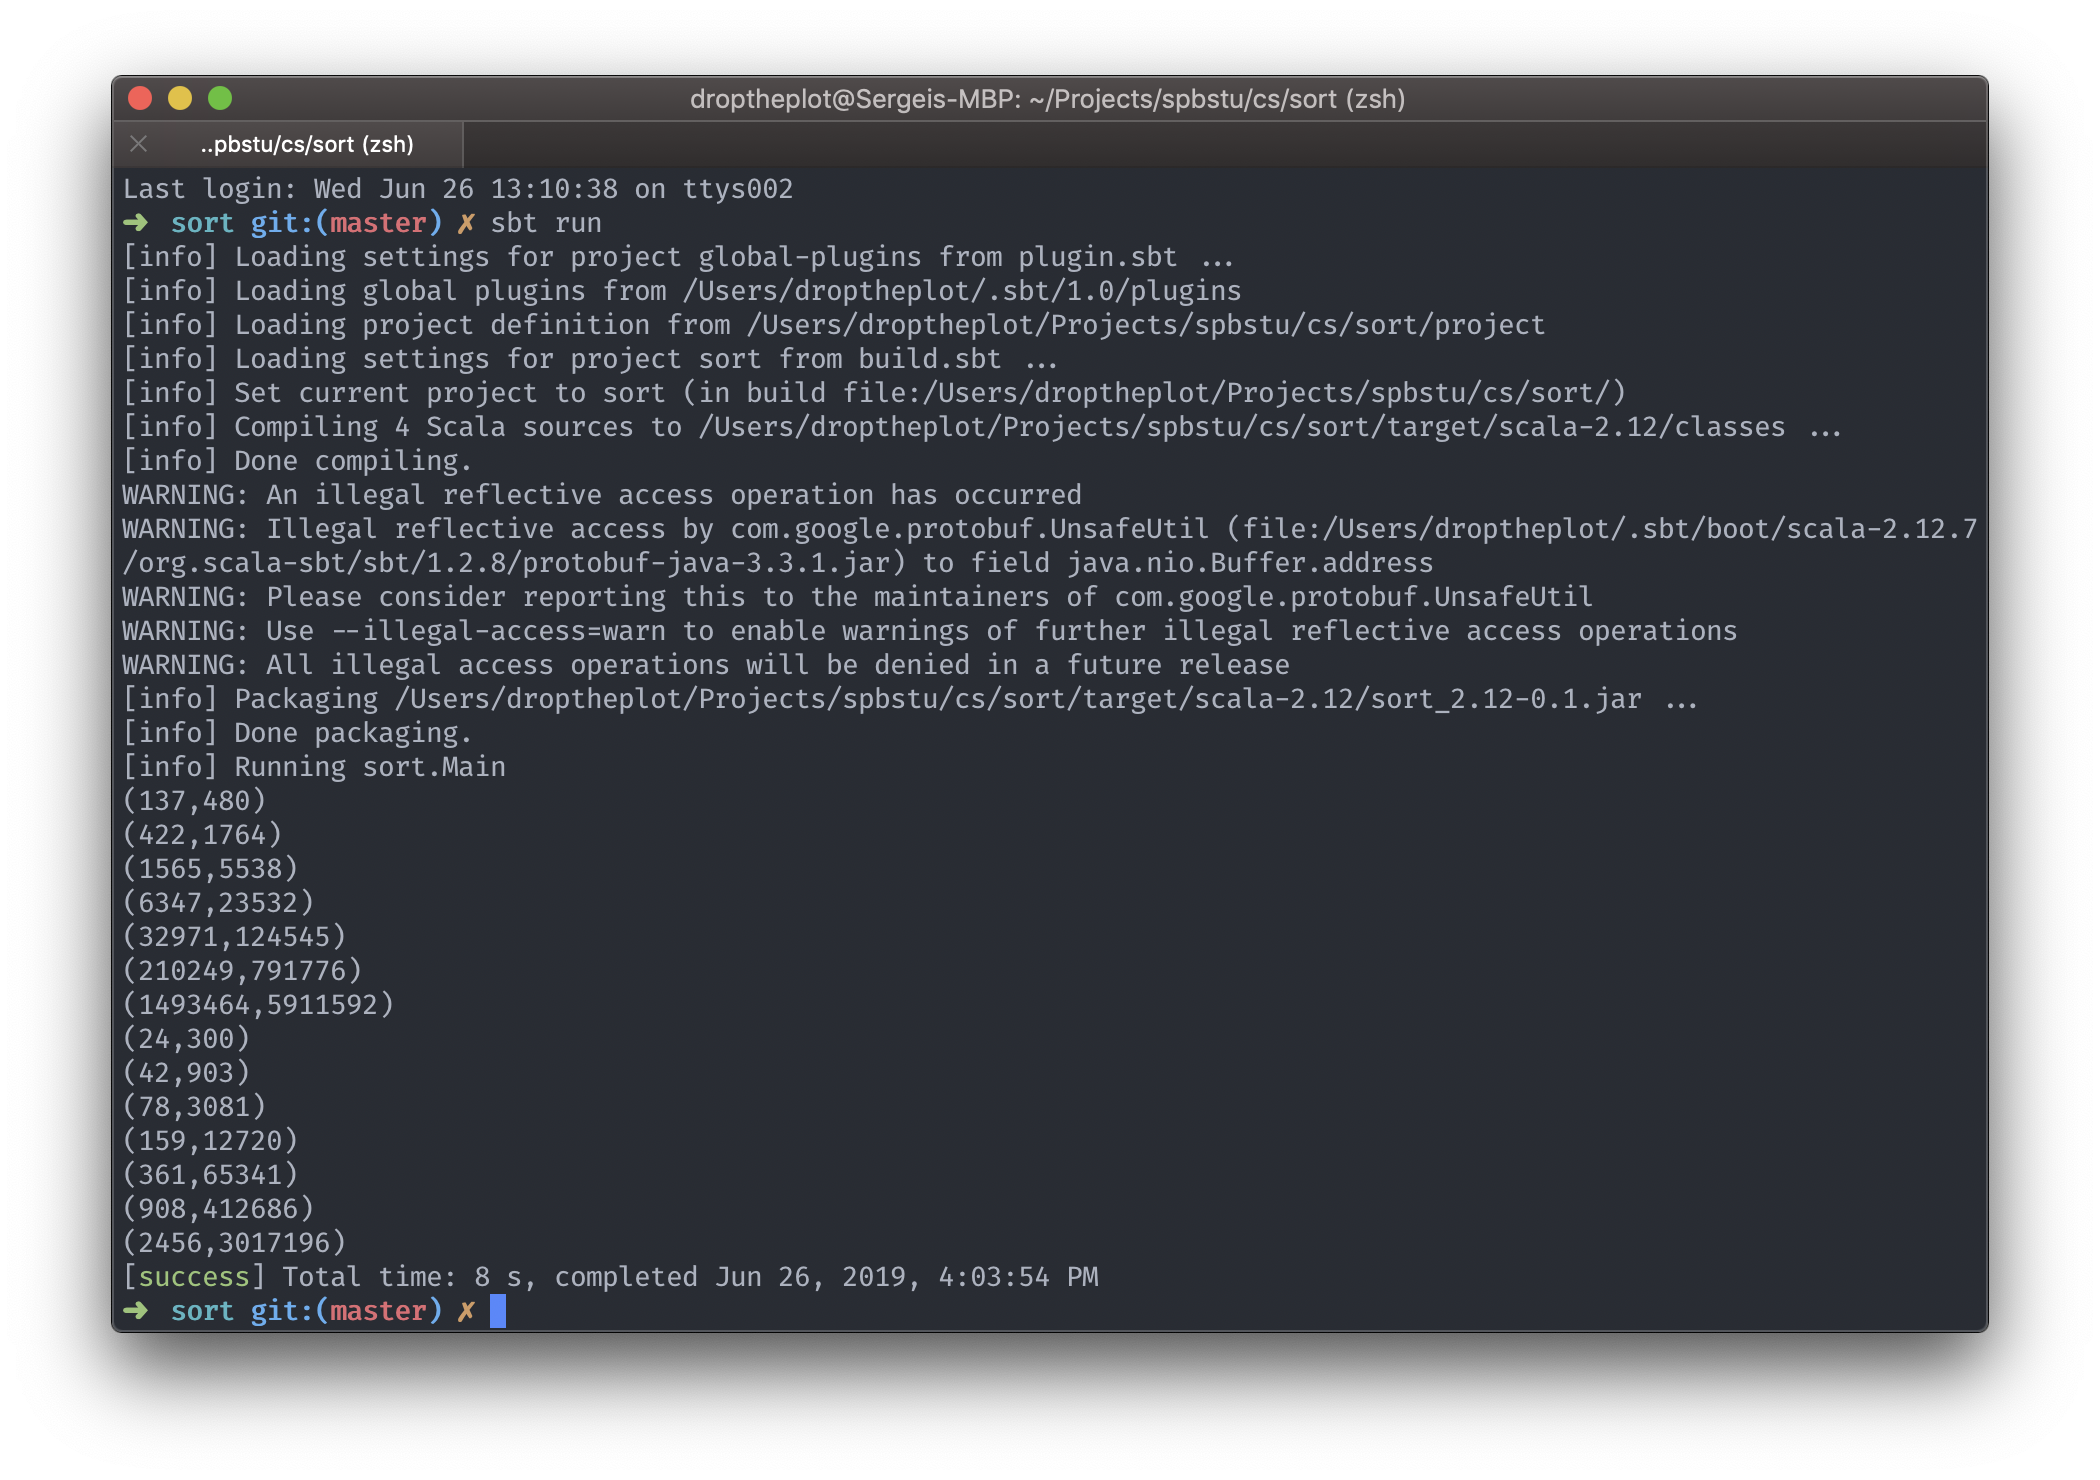
\includegraphics[width=1.2\textwidth]{example}}
\caption{Пример выполнения программы}
\end{figure}

\section{Блок-схема}

\begin{figure}[!htb]
\centerline{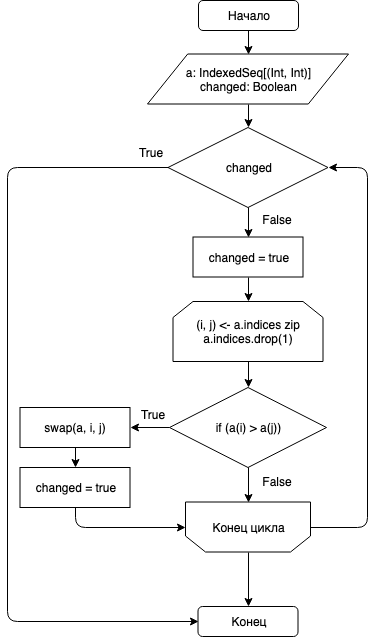
\includegraphics[width=0.7\textwidth]{flowchart}}
\caption{Блок-схема сортировки пузырьком}
\end{figure}

\section{Исходный код}

\subsection{Main.scala}

\lstinputlisting[language=scala]{src/main/scala/sort/Main.scala}

\newpage

\subsection{Impl.scala}

\lstinputlisting[language=scala]{src/main/scala/sort/Impl.scala}

\newpage

\subsection{Bubble.scala}

\lstinputlisting[language=scala]{src/main/scala/sort/Bubble.scala}

\newpage

\subsection{Selection.scala}

\lstinputlisting[language=scala]{src/main/scala/sort/Selection.scala}

\section{Количество сравнений и перестановок в зависимости от размера массива}

\begin{figure}[!htb]
\centerline{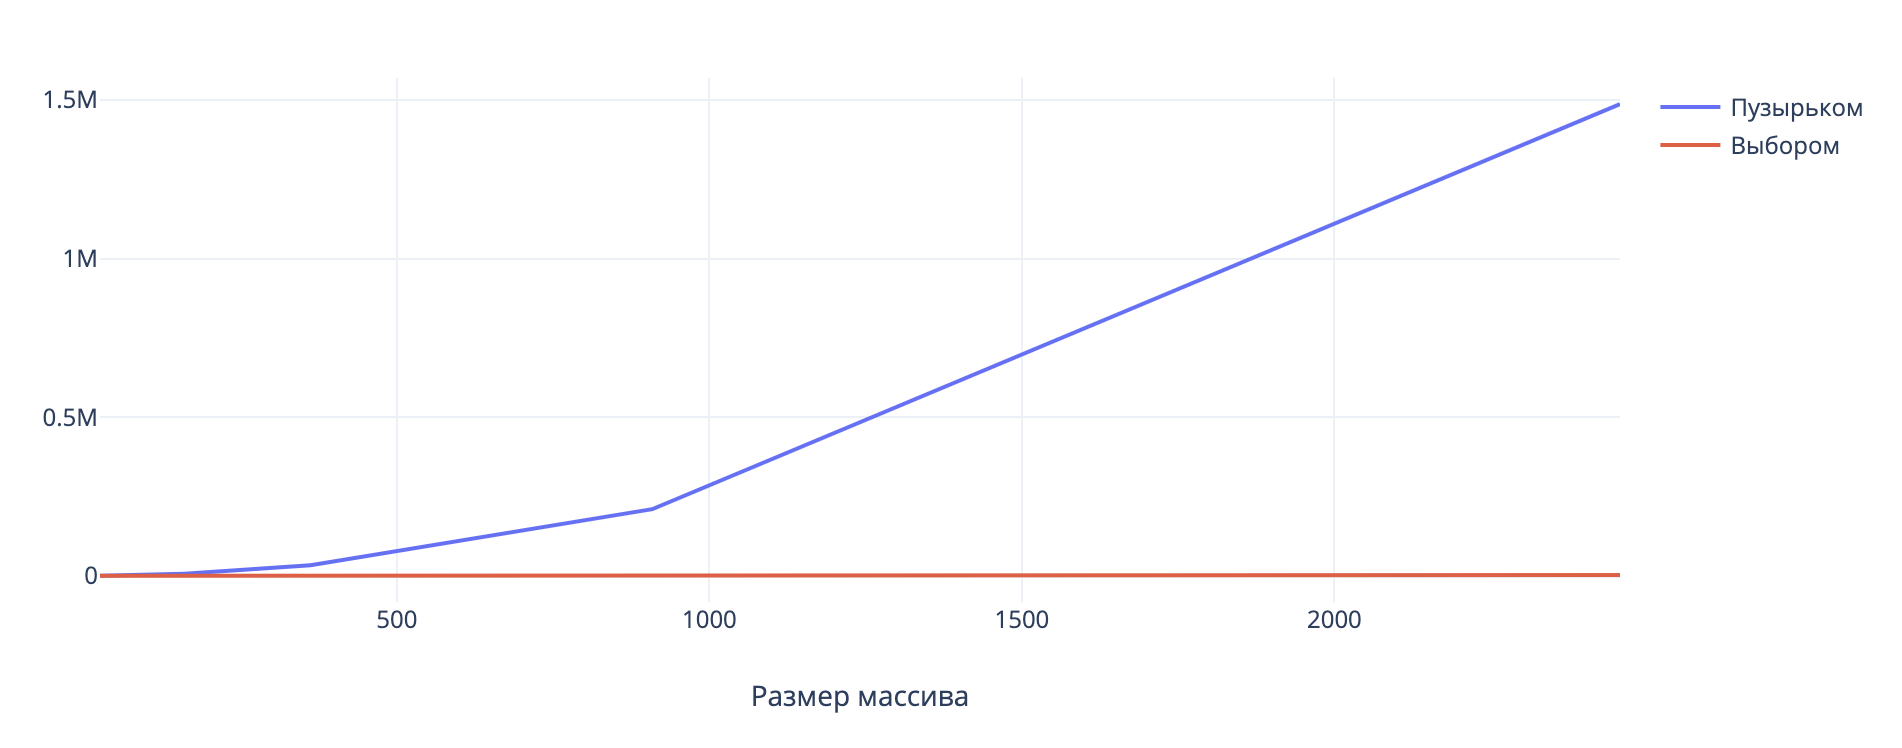
\includegraphics[width=1\textwidth]{swaps}}
\caption{Количество перестановок}
\end{figure}

\begin{figure}[!htb]
\centerline{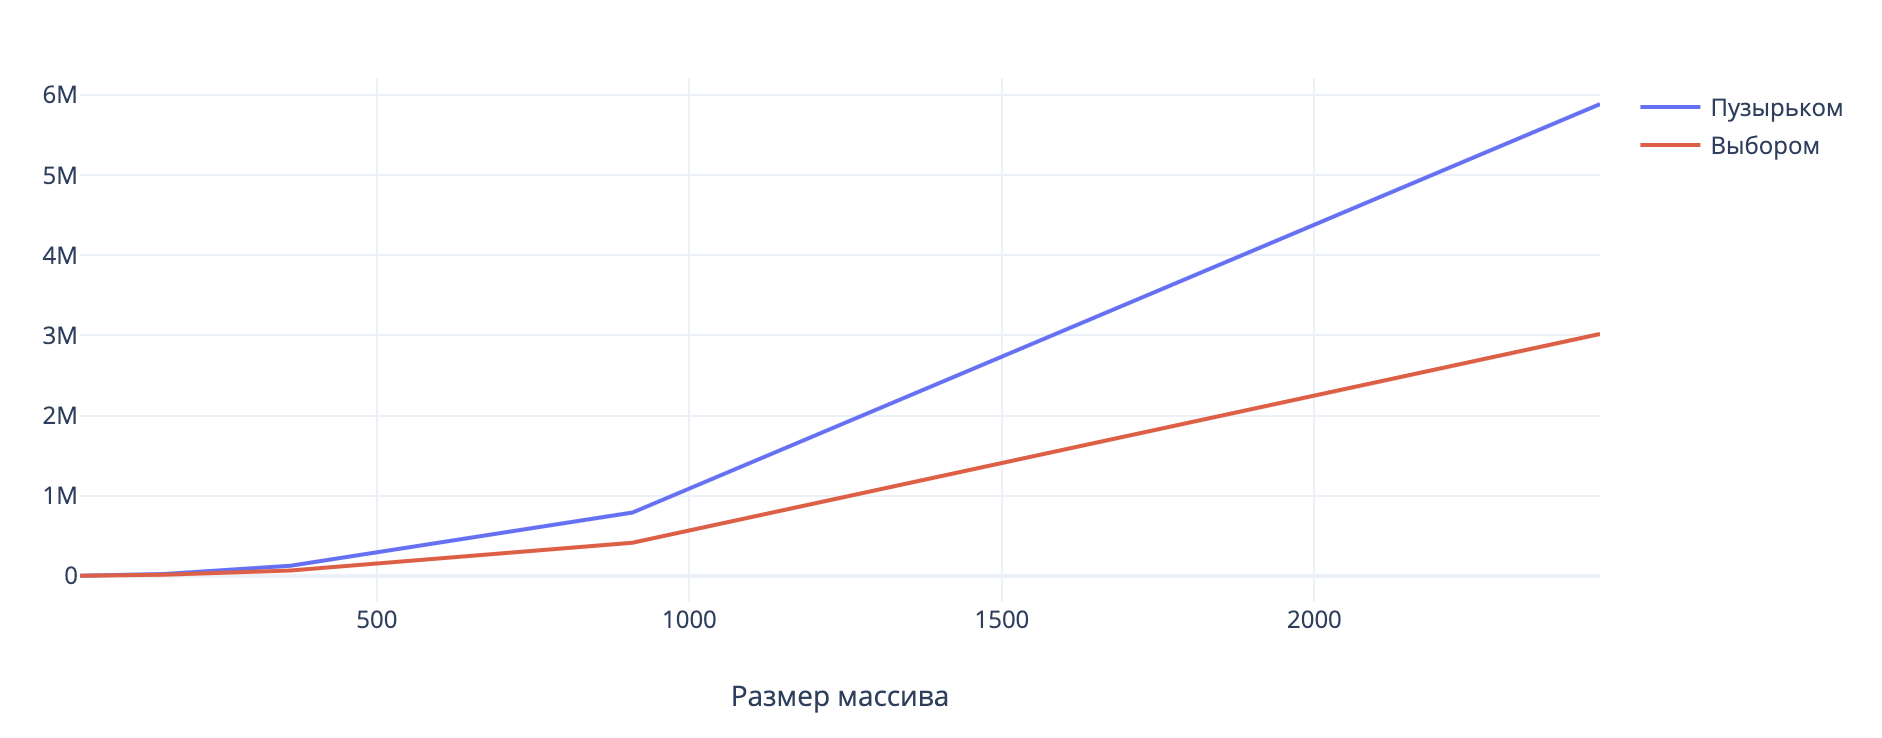
\includegraphics[width=1\textwidth]{comparisons}}
\caption{Количество сравнений}
\end{figure}

\section{Вывод}

В результате решения задачи я обнаружил что сортировка выбором требует меньше сравнений и значительно меньше перестановок, чем сортировка пузырьком.

\end{document}
